\documentclass[crop,tikz]{standalone}
\usetikzlibrary{shapes}
\usetikzlibrary{arrows}
\usetikzlibrary{positioning}
\usepackage{makecell}

\begin{document}
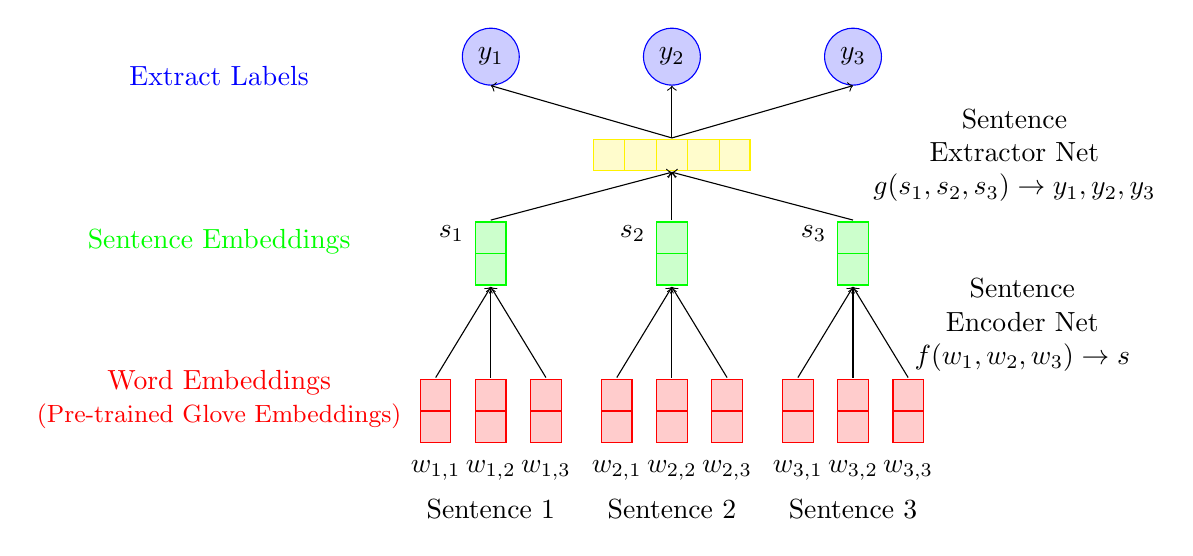
\begin{tikzpicture}[
  hid/.style 2 args={
    rectangle split,
    draw=#2,
    rectangle split parts=#1,
    fill=#2!20,
    outer sep=.25mm},
  mlp/.style 2 args={
    rectangle split,
    rectangle split horizontal,
    draw=#2,
    rectangle split parts=#1,
    fill=#2!20,
    outer sep=.25mm}
]

 % Comment out this line to remove border.
% \draw[draw=black] (0, 6) rectangle (10, 0);

 \node[hid={2}{red}] (w11) at (1,1) {};
 \node[hid={2}{red}] (w12) at (1.7,1) {};
 \node[hid={2}{red}] (w13) at (2.4,1) {};
 \node[] (wl11) at (1,.25) {$w_{1,1}$};
 \node[] (wl12) at (1.7,.25) {$w_{1,2}$};
 \node[] (wl13) at (2.4,.25) {$w_{1,3}$};
 \node[hid={2}{green}] (s1) at (1.7,3) {};
 \draw[->] (w11.north) -- (s1.south);
 \draw[->] (w12.north) -- (s1.south);
 \draw[->] (w13.north) -- (s1.south);

 \node[] (l1) at (1.7,-.25) {Sentence 1};
 \node[] (l1) at (4,-.25) {Sentence 2};
 \node[] (l1) at (6.3,-.25) {Sentence 3};

 \node[hid={2}{red}] (w21) at (3.3,1) {};
 \node[hid={2}{red}] (w22) at (4,1) {};
 \node[hid={2}{red}] (w23) at (4.7,1) {};
 \node[] (wl21) at (3.3,.25) {$w_{2,1}$};
 \node[] (wl22) at (4,.25) {$w_{2,2}$};
 \node[] (wl23) at (4.7,.25) {$w_{2,3}$};
 \node[hid={2}{green}] (s2) at (4,3) {};
 \node (sl2) at (1.2,3.25) {$s_1$};
 \node (sl2) at (3.5,3.25) {$s_2$};
 \node (sl2) at (5.8,3.25) {$s_3$};
 \draw[->] (w21.north) -- (s2.south);
 \draw[->] (w22.north) -- (s2.south);
 \draw[->] (w23.north) -- (s2.south);

 \node[hid={2}{red}] (w31) at (5.6,1) {};
 \node[hid={2}{red}] (w32) at (6.3,1) {};
 \node[hid={2}{red}] (w33) at (7,1) {};
 \node[] (wl31) at (5.6,.25) {$w_{3,1}$};
 \node[] (wl32) at (6.3,.25) {$w_{3,2}$};
 \node[] (wl33) at (7,.25) {$w_{3,3}$};
 \node[hid={2}{green}] (s3) at (6.3,3) {};
 \draw[->] (w31.north) -- (s3.south);
 \draw[->] (w32.north) -- (s3.south);
 \draw[->] (w33.north) -- (s3.south);
     
 \node[circle, draw=blue, fill=blue!20,minimum size=5mm] (y1) at (1.7,5.5) {$y_1$};
 \node[circle, draw=blue, fill=blue!20,minimum size=5mm] (y2) at (4.,5.5) {$y_2$};
 \node[circle, draw=blue, fill=blue!20,minimum size=5mm] (y3) at (6.3,5.5) {$y_3$};

 \node[mlp={5}{yellow}] (h) at (4,4.25) {};
 \draw[->] (s1.north) -- (h.south);
 \draw[->] (s2.north) -- (h.south);
 \draw[->] (s3.north) -- (h.south);
 \draw[->] (h.north) -- (y1.south);
 \draw[->] (h.north) -- (y2.south);
 \draw[->] (h.north) -- (y3.south);

 \node[red] at (-1.75,1.15) {\makecell{Word Embeddings\\\small(Pre-trained Glove Embeddings)}};
 \node[green] at (-1.75,3.15) {Sentence Embeddings};
 \node[blue] at (-1.75,5.25) {Extract Labels};
 \node at (8.45,2.1) {\makecell{Sentence\\Encoder Net\\$f(w_1,w_2,w_3) \rightarrow s$}};
 \node at (8.35,4.25) {\makecell{Sentence\\Extractor Net\\$g(s_1,s_2,s_3)\rightarrow y_1,y_2,y_3$}};


%      \node at (0.4,-.75) {Sentence 1};
%      \node at (4.9,-.75) {Sentence 2};
%      \node at (8.9,-.75) {Sentence 3};
%      \node (w1) at (0,0)
%      {\large $\textsc{Enc}\left(w^{(1)}_1,
%         w^{(1)}_2, w^{(1)}_3 \right)$};
%
%      \node (w2) at (4.5,0)
%      {\large $\textsc{Enc}\left(w^{(2)}_1, 
%         w^{(2)}_2, w^{(2)}_3  \right)$};
%      \node (w3) at (8.6,0)
%      {\large $\textsc{Enc}\left(w^{(3)}_1, 
%         w^{(3)}_2 \right)$};
%
%      \node (s1) at (3,2) {\large $s_1$};
%      \node (s2) at (4,2) {\large $s_2$};
%      \node (s3) at (5,2) {\large $s_3$};
%
%        \draw[->,thick] (w1.north) -- (s1.south);
%        \draw[->,thick] (w2.north) -- (s2.south);
%        \draw[->,thick] (w3.north) -- (s3.south);
%        \node (ext) at (3.6,2) {\large $\textsc{Ext}\Big( 
%        \quad\quad\quad\;\;\;\;\;\;\;\;\;\;\; \Big)$};
%        \node (y1) at (3,3.5) {\large $y_1$};
%        \node (y2) at (4,3.5) {\large $y_2$};
%        \node (y3) at (5,3.5) {\large $y_3$};
%        \draw[->,thick] (s1.north) -- (y1.south);
%        \draw[->,thick] (s2.north) -- (y2.south);
%        \draw[->,thick] (s3.north) -- (y3.south);
%
%
%


















% \foreach \step in {1,...,3} {
%   \node (ie\step) at (1.1*\step - 3.3, -.18) {$s_\step$};
%   \node[hid={2}{green}] (se\step) at (1.1*\step - 3.3, .5) {};    
%   \node[hid={2}{orange}] (he\step) at (1.1 *\step - 3.3, 1.75) {};    
%   \draw[->] (se\step.north) -> (he\step.south);
% } 
%
% \node[rotate=90,orange] at (-2.85, 1.75) {\textbf{Encoder}};
% \node[rotate=-90,yellow] at (3.95, 1.75) {\textbf{Decoder}};
%
% \foreach \step in {1,...,3} {
%   \node (id\step) at (1.1*\step, -.18) {$s_\step$};
%   \node[hid={2}{green}] (sd\step) at (1.1*\step, .5) {};    
%  
%   \node[hid={2}{yellow}] (hd\step) at (1.1 *\step, 1.75) {};    
%   \draw[->] (sd\step.north) -> (hd\step.south);
%
%   \node[mlp={2}{yellow}] (g\step) at (1.1 *\step, 3.0) {};    
%   \node[circle, draw=blue, fill=blue!20,minimum size=5mm] (y\step) 
%       at (1.1 *\step, 3.75) {};
%   \node at (1.1 *\step, 3.75) {$y_\step$};    
%   \draw[->] (g\step.north) -> (y\step.south);
%   \draw[->] (hd\step.north) -> (g\step.south);
%   \node[circle,fill,inner sep=1.25pt] (t\step) at (1.1 * \step, 2.45) {};
% }
%
%
% \draw[-] (he1.north) to [out=90,in=180] (-1.85, 2.55) to (0.55, 2.55) 
%    to [out=0,in=180] (t1.west); 
% \draw[-] (he2.north) to [out=90,in=180] (-0.75, 2.45) to (0.55, 2.45) 
%    to [out=0,in=180] (t1.west); 
% \draw[-] (he3.north) to [out=90,in=180] (0.35, 2.35) to (0.55, 2.35) 
%    to [out=0,in=180] (t1.west); 
% \draw[-] (t1.east) to (t2.west);
% \draw[-] (t2.east) to (t3.west);
%
% \foreach \last/\next in {1/2, 2/3} {
%   \draw[->] (he\last.east) -> (he\next.west);
%   \draw[->] (hd\last.east) -> (hd\next.west);
% }
% \draw[->] (he3.east) -> (hd1.west);


\end{tikzpicture}
\end{document}
